%!TEX root = ../3dchapter.tex

\setchapterpreamble[u]{\margintoc}

\graphicspath{{bim/}}
\renewcommand*{\thelesson}{7.2}

\chapter{Building information modelling}%
\label{chap:bim}

Building information modelling (BIM) is a somewhat fuzzy concept that means different things to different people.
Broadly speaking, it involves the creation and use of detailed digital 3D models of buildings or infrastructure in a way that supports their design and construction, but hopefully also extending to their planning, operation, maintenance, refurbishing and/or demolition.

In industry, this is commonly seen as improving existing processes (\eg\ minimising errors during design and construction), and so the 3D models are only important insofar as they support these processes.
By contrast, a common academic/government view is that BIM is mainly about the 3D models themselves, and thus it is important that they reflect the real situation as much as possible.
In this latter view, the improved processes and new applications are simply the result of using these models in a smart way.

\section{How BIM came to be}

Traditionally, the design of buildings and infrastructure mostly relied on technical drawings on paper, often as a combination of more engineering-focused 2D cross-sections and floor plans, with more visual drawings (\eg\ architectural sketches) that showed an overview of project as 2D perspective views, either in a stylised or in a realistic way.
These were sometimes supplemented with 3D physical models (\ie\ maquettes), but they were created much less frequently than the 2D drawings upon which they were based.

When these design processes were (partly) transferred to computers, it mostly meant the use of 2D computer-aided design (CAD) software to create the technical drawings and the use of general-purpose graphics editing software for the other views.
While this simplified many tasks (\eg\ iterating to make small changes and printing new versions), it is worth noting that the use of these kinds of software did not fundamentally change the nature of designing a building, or of using the archived versions of such designs for later purposes (\eg\ locating pipes and wires), which were most likely only stored in print anyway.

BIM is often considered as an evolution from these CAD-based processes, which is partly true, but it is also a very different way to model buildings and infrastructure.
This is mainly because it models a building or infrastructure project as a single model composed of a large set of 3D objects, as opposed to a series of unconnected 2D drawings showing different views of subsets of these objects.
The kind of technical drawings that were made before are still common, but they can be semi-automatically generated from the BIM model using software.

The objects in a BIM model include the 3D structural elements that a building is composed of (\eg\ beams, columns, stairs and windows) with their accompanying relevant attributes (\eg\ the materials they are made of and their properties), as well as more abstract elements that represent the project itself (\eg\ construction timelines and costs).
There is also a large number of relations between the objects, which are often used by software to support smart editing features, such as keeping sets of related objects together when one of them is moved.

Note that a key aspect of BIM is that it focusses on volume-filling physical objects (Figure~\ref{fig:volumetric}), such as walls, whereas GIS representations instead tend to model the objects' outer surfaces (\eg\ wall surfaces) and the voids between them (\eg\ rooms).
This means that BIM models and usually more detailed and have semantics that are more meaningful for some purposes (\eg\ construction or refurbishing), but 3D GIS models have higher-level semantics that are easier for many applications (\eg\  navigation and spatial analyses).

\begin{figure}
\centering
\includegraphics[width=0.6\linewidth]{figs/volumetric.pdf}
\caption{BIM models focus on volumetric physical elements (centre), whereas 3D GIS models focus on semantic surfaces (left) and the voids between them (right).}%
\label{fig:volumetric}
\end{figure}

\subsection{Use of BIM and common terminology}

BIM was originally focussed on the design of buildings, but its reach has expanded significantly in recent years and is continuing to do so in a number of ways.
Firstly, it is attempting to cover all sorts of non-building infrastructure projects as well, including roads, railways, bridges, tunnels, waterways, utility and communication networks, which together with buildings are often known as \emph{assets}.
Secondly, it also aims to support all the stages of the lifecycle of an asset using the same base data, including its planning (with the help of GIS data), design, construction, operation, maintenance, refurbishing and demolition.
These stages will likely involve different software, \eg\ specialised building design and asset management software; and it will also likely involve different people, \eg\ architects, surveyors, civil engineers, etc.

Relevant to this, some software vendors and organisations (\eg\ the American Institute of Architects and the UK BIM Task Group) have come up with the concept of the level of development (LOD) of a BIM model, which is equivalent to the concept of level of detail (also LOD or LoD) in GIS\@.
While both terms are directly related to how abstract a model is, and indirectly to how complex the geometries in it are, the two terms are somewhat different.
Different LoDs in GIS usually model the same features at the same time, but they are captured at or generalised to different levels of detail.
Different LODs in a BIM model instead show the same asset at the different stages that it goes through, from its conception (as a rough ketch or even with no geometry), and gaining more detail as it passes through its design and to its construction.
Ideally, this extends to modification of the model to reflect its as-built state, which can be then used for asset management and other applications.
The exact terms used for different BIM LODs differ, but a common scheme is from LOD 100 (concept), LOD 200 (design during development), LOD 300 (detailed design to calculate materials and costs), LOD 400 (construction) and LOD 500 (asset management).
Other schemes use smaller numbers, such as 1 to 7 in the United Kingdom, or use the same hundreds-series numbers but with different definitions.

Another important set of terms is related to the dimensions in BIM, which are commonly used but they are used inconsistently\@.
In this, practitioners and software vendors very often refer to 4D BIM, which means that a model includes time information, generally in the context of construction scheduling.
Note however that this information might not be in a convenient format, \eg\ a linked Word file with a textual description.
Other dimension definitions sometimes refer to 5D BIM, which usually means a model with cost information.
Finally, different people use 6D or 7D BIM to refer to various other aspects (sustainability, facility management, and delivery of as-built models among others), but the definitions for these are very inconsistent.

Apart from the core applications of BIM in managing a building's lifecycle mentioned above, it is worth noting that there are also many new possibilities that are currently being studied, such as the automatic conversion of BIM models into GIS-ready models that can be integrated into 3D city models, applying environmental analyses directly on BIM models (\eg\ shadow analyses), improving the sustainability of buildings (green BIM), using BIM models to automate building permit issuing, and as will be further discussed in this course, the integration of BIM models with GIS data (GeoBIM).

\section{IFC}

BIM is an industry-dominated field, and software-specific file formats are still the main way in which files are exchanged, such as using the native formats of Autodesk's Revit\footnote{\url{https://www.autodesk.com/products/revit/overview}} and Graphisoft's ArchiCAD\footnote{\url{https://www.graphisoft.com/archicad/}} (BIMx).
However, such formats are only well supported by their corresponding software programs, which leads to interoperability problems when exchanging files.

As a way to solve this problem, the buildingSMART consortium, which notably includes a number of software companies (including Autodesk and the Graphisoft-owning Nemetschek Group)\footnote{\url{https://www.buildingsmart.org/members/member-directory/}}, created the industry foundation classes (IFC)\footnote{\url{http://www.buildingsmart-tech.org/specifications/ifc-releases}} as an open data model for the exchange of BIM models.
IFC has been further standardised as ISO 16739~\citep{ISO16739:2013} with its geometry definitions in ISO 10303~\citep{ISO10303:2014}.

IFC files are often large (hundreds of MBs), and their structure is rather complex.
They can contain many types of classes (130 defined types, 217 enumeration types, 60 select types, 816 entities, 47 functions, 2 rules, 415 property sets, 93 quantity sets and 1697 individual properties in IFC 4.2\footnote{\url{https://standards.buildingsmart.org/IFC/DEV/IFC4_2/FINAL/HTML/}}), which are defined using the EXPRESS data modelling language.
Among others, there are several classes to model actors (\eg\ people and organisations), controls (\eg\ specifications, regulations, schedules and other requirements), processes (\eg\ actions during construction), products (\eg\ physical building elements and other spatially defined objects), the project itself (\eg\ where it is placed), and resources (\eg\ cost, materials and equipment), as well as groups of other classes (\eg\ those having a common purpose).
In the rest of this handout, we will mostly focus on products.

\subsection{Encoding}

The most common encoding of IFC files is the STEP Physical File (SPF), which is a plain text format that is reasonably compact, easy to parse by a computer and human readable (Figure~\ref{fig:step}).
It is also defined in the ISO 10303 standard.
Files with this encoding have the extension \texttt{.ifc}.

\lstset{basicstyle=\footnotesize\ttfamily,breaklines=true}
\begin{figure}
\begin{lstlisting}[frame=single]
#365= IFCDIRECTION((1.,0.,0.));
#367= IFCDIRECTION((0.,0.,1.));
#369= IFCCARTESIANPOINT((0.,0.,0.));
#371= IFCAXIS2PLACEMENT3D(#369,#367,#365);
#372= IFCDIRECTION((0.766044443119,0.642787609687));
#374= IFCGEOMETRICREPRESENTATIONCONTEXT($,'Plan',3,1.00000000000E-5,#371,#372);
#375= IFCGEOMETRICREPRESENTATIONSUBCONTEXT('Box','Plan',*,*,*,*,#374,$,.PLAN_VIEW.,$);
#377= IFCCARTESIANPOINT((-3.,-3.,-1.));
#379= IFCBOUNDINGBOX(#377,18.,16.,1.);
#380= IFCSHAPEREPRESENTATION(#375,'Box','BoundingBox',(#379));
#383= IFCPRODUCTDEFINITIONSHAPE($,$,(#355,#380));
#389= IFCSITE('0KMpiAlnb52RgQuM1CwVfd',#12,'Gelaende','Ebenes Gelaende','LandUse',...
#400= IFCRELAGGREGATES('1GO86xgv8B470LzUwG9dnQ',#12,$,$,#66,(#389));
#406= IFCPROPERTYSINGLEVALUE('BuildingHeightLimit',$,IFCPOSITIVELENGTHMEASURE(9.),$);
#407= IFCPROPERTYSINGLEVALUE('GrossAreaPlanned',$,IFCAREAMEASURE(0.),$);
#408= IFCPROPERTYSET('1pzemvk20um3F9bx64I1e9',#12,'Pset_SiteCommon',$,(#406,#407));
#412= IFCRELDEFINESBYPROPERTIES('2w5hE3w6ce8Clm81uDvALx',#12,$,$,(#389),#408);
#416= IFCQUANTITYLENGTH('GrossPerimeter',$,$,0.,$);
#419= IFCQUANTITYAREA('GrossArea',$,$,0.,$);
\end{lstlisting}
\caption{Excerpt of a typical IFC file encoded in STEP\@.
After a short metadata header, a file consists of a series of lines, where every line starts with a hash sign (\#), followed by the definition of an entity.
An entity is assigned a numeric ID, followed by an equals sign (=), the name of the entity, and a tuple of its parameters.
These parameters can be empty (\texttt{\$}), a number, a list (a comma separated list enclosed by parentheses), a text string (enclosed by single quotes), or the ID of another entity, among others.}%
\label{fig:step}
\end{figure}

In addition to STEP files, there is also an XML encoding of the standard (IFC-XML) with file extension \texttt{.ifcXML}, as well as a zipped version of the other encodings with extension \texttt{.ifcZIP}.
These two are less convenient due to the large file of XML files and the need to uncompress its zipped version.
They are thus rarely used in practice.

\subsection{How objects are modelled}

Physical elements in IFC (\ie\ \texttt{IfcElement}) are usually modelled separately using a local coordinate system that is defined per object (as opposed to the national or regional coordinate systems used in GIS).
This reflects the fact that in BIM and CAD, objects are generally modelled independently before later being fitted together.
In practice, this means that the location of an independently-modelled element is defined by a hierarchy of transformations.
For example, these levels can correspond to the levels in a decomposition structure (typically a site, project, building and individual floors), or link an element to another element (a dependent element linked to one it is attached to).

In concrete terms, a product in IFC (\ie\ \texttt{IfcProduct}, which is a superclass of \texttt{IfcElement}), is linked to a geometry (\ie\ \texttt{IfcProductRepresentation}) and to the local coordinate system that defines its location (\ie\ \texttt{IfcObjectPlacement}).
The latter can be absolute (\ie\ defined with respect to the whole project's coordinate system) or relative (\ie\ defined with respect to another product).

\subsection{Geometry}

The geometry of a physical element can be created using a variety of representation paradigms:
\begin{description}
  \item[Primitive instancing:] an object is represented based on a set number of predefined parameters (Figure~\ref{fig:parametric}).
  IFC uses this paradigm to define various forms of 2D profiles (Figure~\ref{fig:profiles}), as well as volumetric objects, such as spheres, cones and pyramids.
  \item[CSG and Boolean operations:] an object is represented as a tree of Boolean set operations (union, intersection and difference) of volumetric objects (Figure~\ref{fig:csg}).
  Half-spaces are often used to cut out the undesired parts of surfaces or volumes.
  \item[Sweep volumes:] a solid can also be defined by a 2D profile (a circle, a rectangle or an arbitrary polygon with or without holes) and a curve along which the surface is extruded (Figure~\ref{fig:sweeps}).
  \item[B-rep:] an object is represented by its bounding surfaces, either triangulated meshes, polygonal meshes or topological arrangements of free-form surfaces (Figure~\ref{fig:brep}).
\end{description}
These paradigms can be used independently or combined with each other in a hierarchy.

\begin{figure}
\begin{lstlisting}[frame=single]
#17079= IFCDIRECTION((1.,0.));
#17081= IFCCARTESIANPOINT((0.,0.));
#17083= IFCAXIS2PLACEMENT2D(#17081,#17079);
#17084= IFCRECTANGLEPROFILEDEF(.AREA.,'',#17083,0.885,2.01);
\end{lstlisting}
\caption{Defining a rectangular profile (\ie\ \texttt{IfcRectangleProfileDef}) parametrically.
The rectangle extends 0.885 units along the x-axis, which is defined by the direction given in its \texttt{IfcAxis2Placement2D} \((1,0)\), and 2.01 units along the y-axis (perpendicular to the x-axis).}%
\label{fig:parametric}
\end{figure}

\begin{figure}
\centering
\begin{subfigure}[b]{0.45\linewidth}
	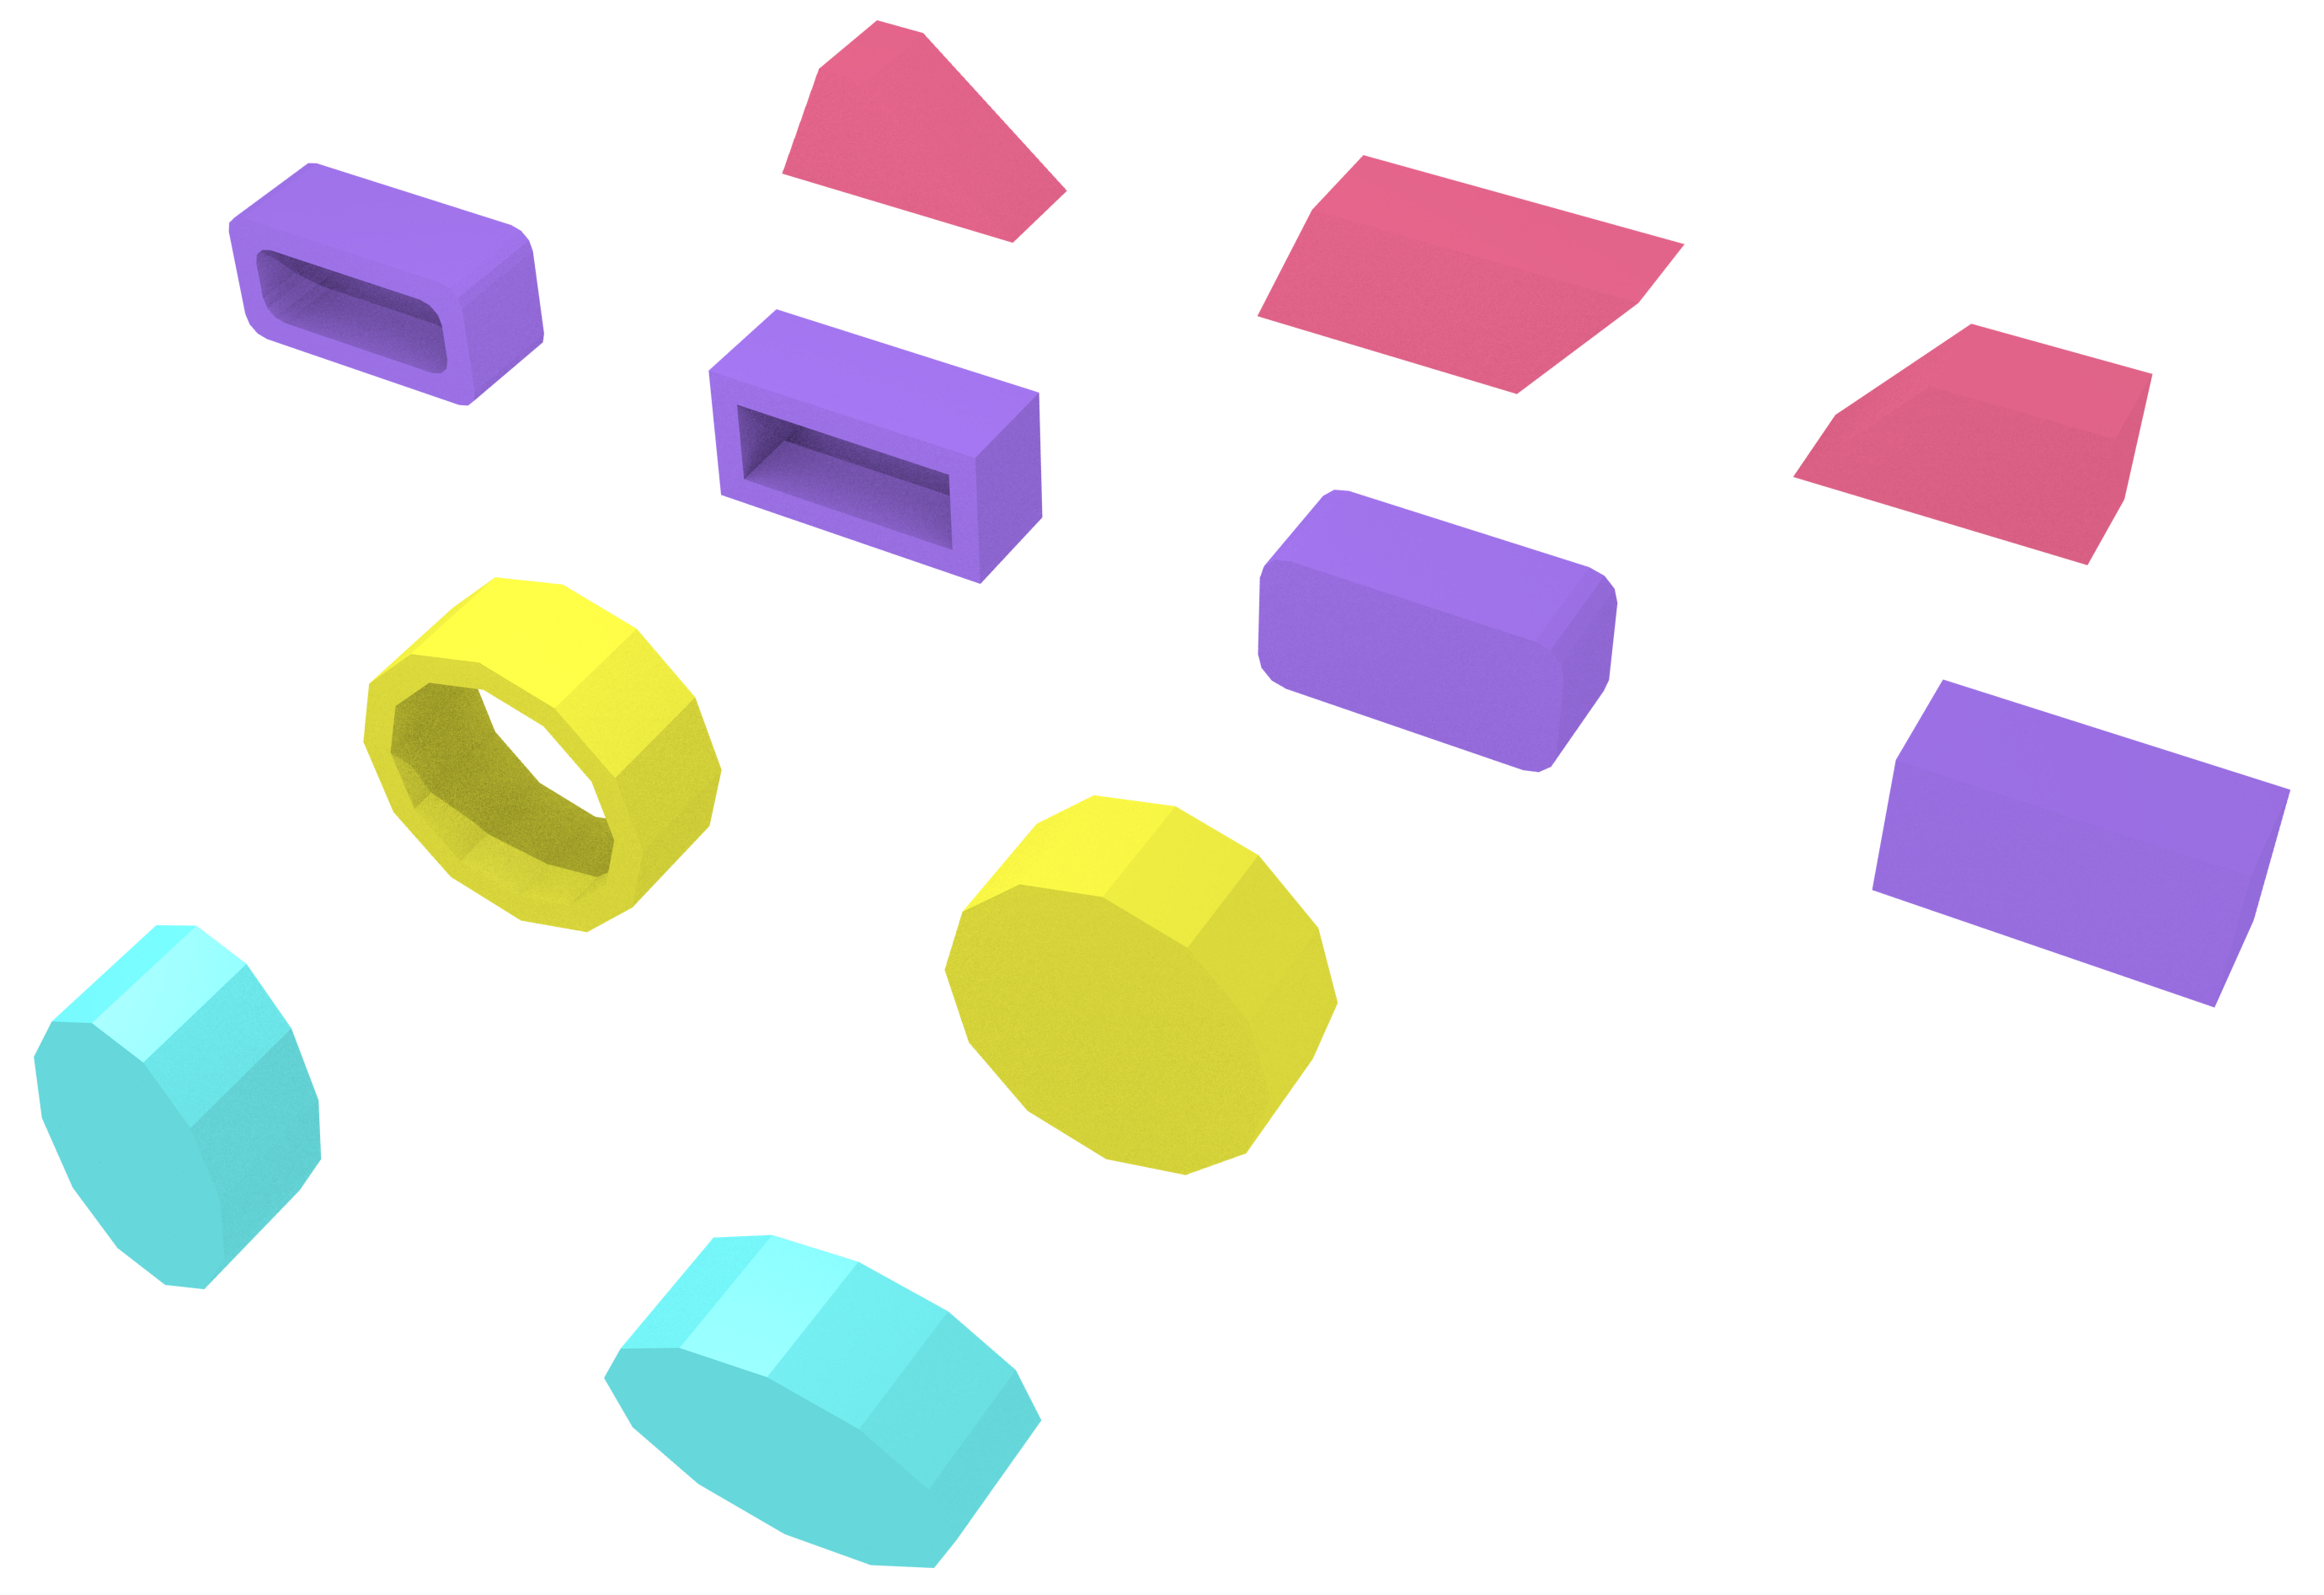
\includegraphics[width=\linewidth]{figs/profiles}%
	\label{subfig:profiles}
\end{subfigure}
\begin{subfigure}[b]{0.45\linewidth}
	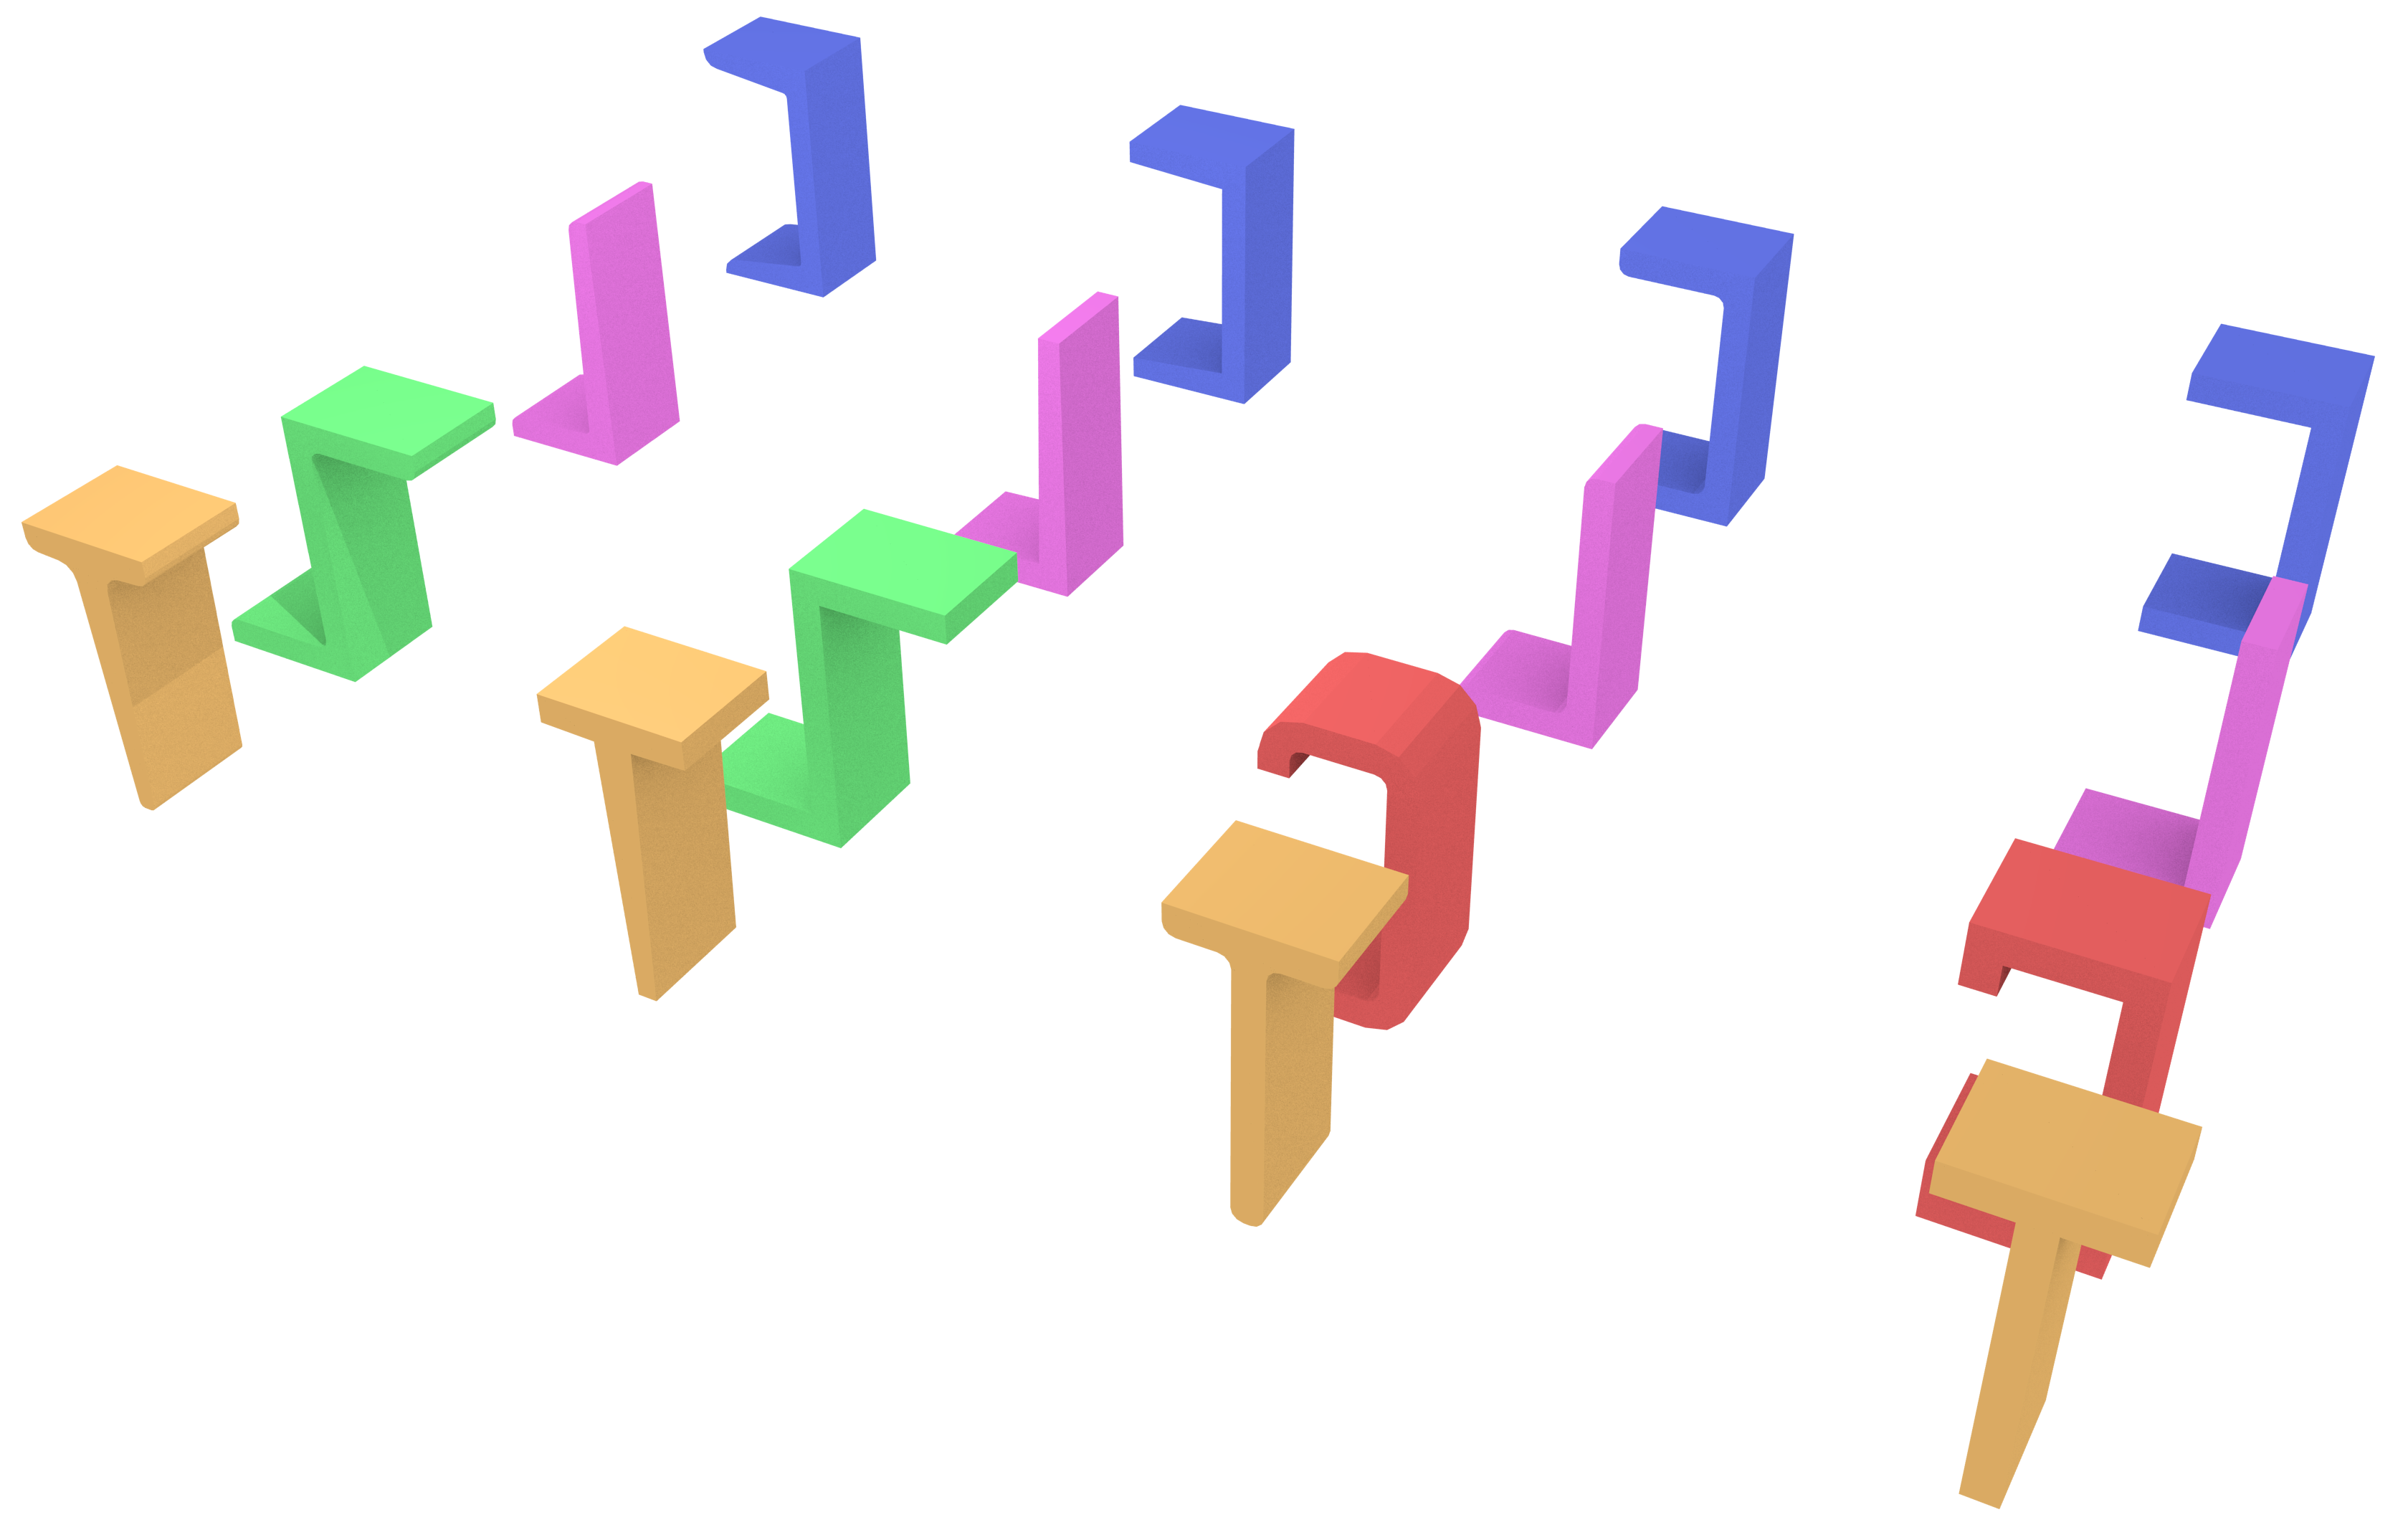
\includegraphics[width=\linewidth]{figs/letter_profiles}%
	\label{subfig:letter-profiles}
\end{subfigure}
\caption{The IFC standard supports parametric instantiated objects, such as these extrusions of (a) shape profiles and (b) letter profiles.}%
\label{fig:profiles}
\end{figure}

\begin{figure}
\begin{lstlisting}[frame=single]
#237=IFCEXTRUDEDAREASOLID(#236,#234,#230,6000.);
#238=IFCDIRECTION((1.,0.,0.));
#239=IFCDIRECTION((-1.,0.,1.));
#240=IFCCARTESIANPOINT((-2500.,0.,3000.));
#241=IFCAXIS2PLACEMENT3D(#240,#239,#238);
#242=IFCPLANE(#241);
#243=IFCHALFSPACESOLID(#242,.F.);
#244=IFCBOOLEANCLIPPINGRESULT(.DIFFERENCE.,#237,#243);
\end{lstlisting}
\caption{Removing part of a volume by subtracting a half-space from it using a Boolean operation.}%
\label{fig:csg}
\end{figure}

\begin{figure}
\centering
\begin{subfigure}[b]{0.45\linewidth}
	\includegraphics[width=\linewidth]{figs/ifc-1}%
	\label{subfig:ifc-1}
\end{subfigure}
\begin{subfigure}[b]{0.45\linewidth}
	\includegraphics[width=\linewidth]{figs/ifc-2}%
	\label{subfig:ifc-2}
\end{subfigure}
\caption{The IFC standard supports objects defined through sweeps, which are defined by (a) an \texttt{IfcPCurve} (black spiral) and a \texttt{SweptArea} (blue disk), in this case resulting in (b) a screw shape.}%
\label{fig:sweeps}
\end{figure}

\begin{figure}
\begin{lstlisting}[frame=single]
#120= IFCCARTESIANPOINT((-3.,13.,0.));
#122= IFCCARTESIANPOINT((12.,10.,0.));
#124= IFCCARTESIANPOINT((15.,13.,0.));
#126= IFCPOLYLOOP((#120,#122,#124));
\end{lstlisting}
\caption{Defining a simple polygon (\ie\ \texttt{IfcPolyLoop}) using B-rep.
Every point is defined as an \texttt{IfcCartesianPoint}, then the polygon is defined by a list of points.}%
\label{fig:brep}
\end{figure}

\subsection{Semantics}

The semantics in an IFC file are stored in two main ways: by using specific entities and by storing them in the attributes of more generic classes.

An example of the first case is given by all the subentities of \texttt{IfcBuildingElement}, including: \texttt{IfcBeam}, \texttt{IfcBuildingElementComponent}, \texttt{IfcBuildingElementProxy}, \texttt{Ifc\-Chim\-ney}, \texttt{Ifc\-Co\-lumn}, \texttt{IfcCovering}, \texttt{IfcCurtainWall}, \texttt{IfcDoor}, \texttt{IfcFooting}, \texttt{IfcMember}, \texttt{IfcPile}, \texttt{Ifc\-Plate}, \texttt{Ifc\-Rai\-ling}, \texttt{IfcRamp}, \texttt{Ifc\-Ramp\-Flight}, \texttt{IfcRoof}, \texttt{IfcShadingDevice}, \texttt{IfcSlab}, \texttt{Ifc\-Stair}, \texttt{Ifc\-Stair\-Flight}, \texttt{IfcWall}, and \texttt{Ifc\-Win\-dow}.
These can be used to represent the different functions that a building element has, although there is also a commonly used generic one (\ie\ \texttt{IfcBuildingElementProxy}) that does not provide this information.
Similar subentities exist in other parts of the standard, such as for distribution elements (\eg\ for heating, cooling, ventilation and plumbing).

Regarding the second case, a good example is given by the various property sets of IFC\@.
For instance, a building's use can be defined using the property set \texttt{Pset\_BuildingUse}, which includes things like its market category (\eg\ residential or commercial).
Another example is given in Figure~\ref{fig:pset}, where custom properties are defined in order to store specific semantics of a model.

\begin{figure}
\begin{lstlisting}[frame=single]
#991622=IFCPROPERTYSINGLEVALUE('End Extension Calculation',$,IFCLENGTHMEASURE(3000.),$);
#991623=IFCPROPERTYSINGLEVALUE('Material',$,IFCLABEL('NL_01_hout_plaat'),$);
#991624=IFCPROPERTYSINGLEVALUE('Length',$,IFCLENGTHMEASURE(2594.),$);
#991625=IFCPROPERTYSINGLEVALUE('Start Release',$,IFCINTEGER(3),$);
#991626=IFCPROPERTYSINGLEVALUE('End Release',$,IFCINTEGER(1),$);
#991627=IFCPROPERTYSINGLEVALUE('Cut Length',$,IFCLENGTHMEASURE(2594.000000000001),$);
#991628=IFCPROPERTYSINGLEVALUE('Structural Usage',$,IFCINTEGER(10),$);
#991629=IFCPROPERTYSINGLEVALUE('Analyze As',$,IFCINTEGER(1),$);
#991630=IFCPROPERTYSINGLEVALUE('Volume',$,IFCVOLUMEMEASURE(13602936.00000029),$);
\end{lstlisting}
\caption{Defining properties to store the semantics in an IFC model.}%
\label{fig:pset}
\end{figure}

\subsection{Georeferencing}

Properly georeferencing an IFC file makes it possible to link the (local) coordinates inside an IFC model with their corresponding real-world coordinates, and thus to place the model of a single building or construction within the virtual environment.
However, it is important to say that most IFC models are not georeferenced properly (or at all), which is a major issue in practice.

In order to georeference an IFC file, it is possible to use the IFC entity \texttt{IfcSite}, which defines an area where construction works are undertaken, and optionally allows for storage of the real-world location of a project using the \emph{RefLatitude}, \emph{RefLongitude} and \emph{RefElevation} attributes.
The latitude and longitude are defined as angles with degrees, minutes, seconds, and optionally millionths of seconds with respect to the world geodetic system WGS84 (EPSG:4326).
Positive values represent locations north of the equator, west of the geodetic zero meridian (nominally the Greenwich prime meridian) in IFC2x3, or east of the zero meridian IFC4.
Negative values represent locations south of the equator, east of the zero meridian in IFC2x3, or west of the zero meridian in IFC4.
All the components of these angles (\ie\ degrees, minutes, seconds and millionth-seconds of arc) should have the same sign.
According to the IFC standard, the geographic reference given might be the exact location of the origin of the local placement of the \texttt{IfcSite} or it might be an approximate position for informational purposes only.
The elevation is defined according to the datum elevation relative to sea level.

The IFC entity \texttt{IfcGeometricRepresentationContext} is used to define the coordinate space of an IFC model in 3D and optionally the 2D plan of such a model.
This entity can be used to offset the project coordinate system from the global point of origin using the \emph{WorldCoordinateSystem} attribute, it defines the \emph{Precision} under which two given points are still assumed to be identical, and it defines the direction of the \emph{TrueNorth} relative to the underlying coordinate system.
The latter attribute defaults to the positive direction of the y-axis of the \emph{WorldCoordinateSystem}.

\section{Exercises}

\begin{enumerate}

\item
Open a simple IFC file (\eg\ the IfcOpenHouse) in a text editor.
Can you understand the general structure of the file and how the STEP encoding works? 

\item
Find a line that defines an \texttt{IfcAxis2Placement3D}.
With the help of the documentation of that entity in the buildingSMART website, can you understand what it means?

\item
Much like 3D GIS standards like CityGML, IFC files represent a hierarchy.
However, the hierarchy in an IFC file looks much flatter with a simple entity in every line.
What are some advantages and disadvantages of this approach?

\end{enumerate}
